%DAQ_Measuremnt_V
\chapter{First DAQ Measurements: Voltage}

\objectives
{
\item Describe the function of an analog to digital converter, and identify the
	limitations of analog to digital conversion.
\item Calculate the uncertainty in a voltage measurement arising from analog
	to digital conversion.
\item Identify the voltage limits of the Arduino, and how one can avoid
	exceeding those limits.
\item Build a voltmeter using the ADC on an Arduino that can measure 0-5 Volts.
\item Build a voltmeter using the ADC on an Arduino that can measure 0-30 Volts.
}

\review
{
\item Electric potential and voltage.
}

Let's review what we learned last week. When we are making measurements
electronically, we are ultimately measureing voltages.
If the data is not a voltage, we must convert it into a
voltage. We have already converted current into a voltage (using a shunt
resistor). 

What is a voltage? Let's review quickly. 
In the last lab we said that voltage is a measure of
electrical potential energy. It is also likely that you are familiar with 
the word ``voltage'' because we live in a world that
has electricity everywhere. You probably know that your house or apartment
has wires in the walls that carry ``110
Volts'', and you probably realize that ``voltage'' 
is a measure of how much energy there is in the
wires.

For today, the key things for us to remember are (1) that voltage 
is proportional to an electrical potential
energy difference, and (2) that when we measure voltage we are
measuring something proportional to energy.

Because voltage is proportional to a \emph{difference} in electrical
potential energy, a voltage measurement really is a combination of two
measurements. Think of gravitational potential energy. If we ask for the
potential energy difference as Super Guy jumps from the bottom of a building
to the top 
we need two measurements, one at
the bottom and one at the top
(Figure \ref{fig:gravitational_energy_difference}). 
The potential energy difference is then found
by taking the difference in energies at the top and bottom of the building:
\begin{equation*}
\Delta U_{g}=U_{g_{top}}-U_{g_{bottom}}
\end{equation*}
\begin{figure}[htbp!]
\centering
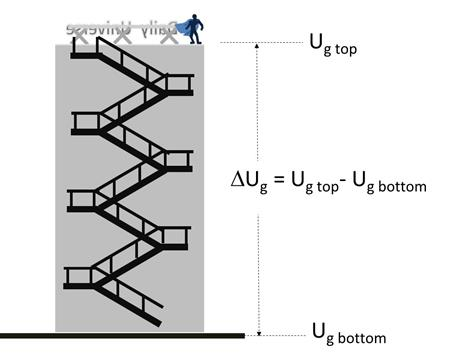
\includegraphics[width=0.5\textwidth]{PH4CAU1I}
\caption[Gravitational potential energy difference.]{Gravitation potential
energy difference is found by taking the difference of potential energies 
between the initial and final position.}
\label{fig:gravitational_energy_difference}
\end{figure}

We will do something very similar in measuring voltages. We will measure the
potential energy at two places. For example, suppose we have an electric
circuit as shown in Figure \ref{fig:voltage_measurement}. 
The circuit is very simple, just
a battery and a resistor. A battery is just a source of electric potential 
energy, and a resistor is just a piece of material that has lots of electrical
friction, or ``resistance'' that makes it
hard for electrons to go through it. If we want to measure the voltage
across the resistor, we have to measure on the top and bottom of the
resistor. That will give us a measurement proportional to the potential
energy difference from one side to the other of the resistor.
\begin{figure}[htbp!]
\centering
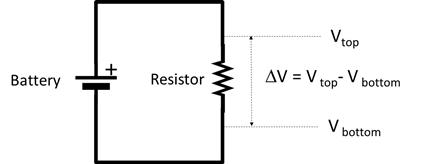
\includegraphics[width=0.5\textwidth]{PH4CAU1J}
\caption[Measuring electric potential energy difference]{Measuring electric
potential energy difference, or voltage. Two measurements are required,
one where the potential is high, and one where the potential is low. 
The voltage is the difference between these two measurements.}
\label{fig:voltage_measurement}
\end{figure}

As we saw in the last lab, most meters that measure voltage (``voltmeters'')
have 
two ``probes''. The meter reads a potential from each probe and completes
the difference calculation internally.
These meters are called \emph{voltmeters} and we used them last week.
In today's world, voltmeters are usually just one function provided by
multimeters.

We learned to use a stand-alone voltmeter in the last lab. Now we also need
to read in voltages in a way that the data can be transferred automatically
to a computer. To do this, we will use the \emph{analog} pins on our
Arduino board.

Before we begin, we need a warning. We absolutely must not wire up the
analog pins on our Arduino backwards! This can (and probably will) destroy
the pin circuitry inside our Arduino. So we will need to be careful in
wiring for this part of our lab. Where this could be a problem a warning
sign (seen in Figure \ref{fig:warning}) will appear in the text, 
just to remind you to be careful! 
You may see quite a few of these in this lab.
\begin{figure}[htbp!]
\centering

\includegraphics[width=0.4\textwidth]{PH4CAU1L}
\caption[Example warning sign]{An example warning sign. Wiring an
Arduino incorrectly can destroy parts of the Arduino. When this is
a possibility, you will see this warning sign.}
\label{fig:warning}
\end{figure}

\section{Building a Voltmeter}

To act like a voltmeter that communicates with a computer, 
the Arduino needs to do three things:
\begin{enumerate}
\item Read the voltage signal.
\item Convert the voltage signal to a number.
\item Send the data to the computer.
\end{enumerate}

Let's look at these in greater detail.

\subsection{Analog Pins on the Arduino}

Analog signals are read at the analog pins on the Arduino. These can be seen in 
Figure \ref{fig:arduino_right}, and are labeled A0 through A5. You will also
note that there are two ground (GND) connections on this side of the Arduino.
When measuring voltages with the Arduino, the wires that we use as our probes 
will go into one of the A0 to A5 pins and into one of the GND pins, or into 
two of the A0 to A5 pins.
\begin{figure}[htbp!]
\centering
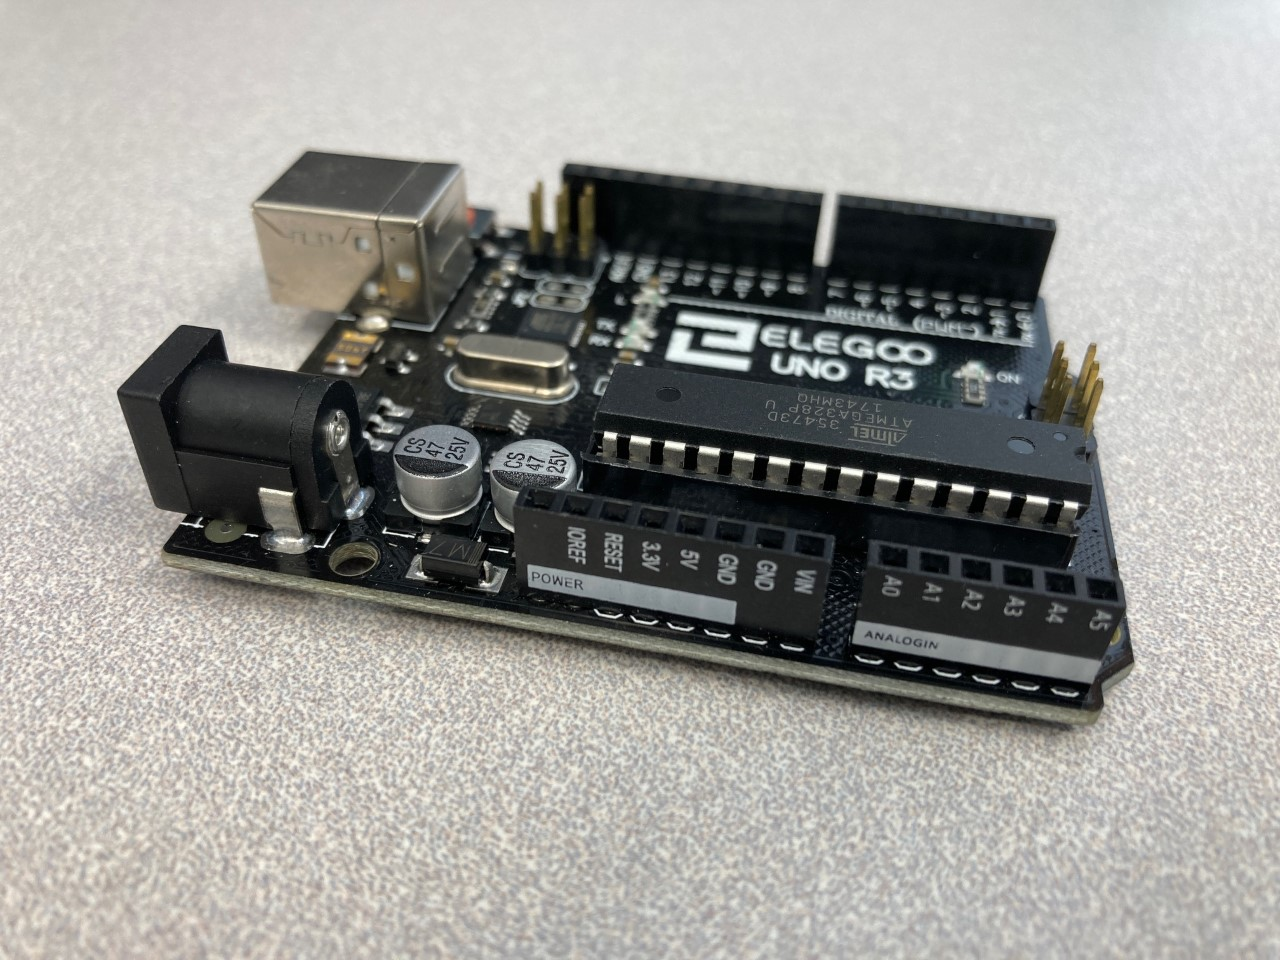
\includegraphics[width=0.8\textwidth]{arduino_right}
\caption[The analog pins on the Arduino]{The analog pins on the Arduino,
seen on the right side and labeled A0 through A5.}
\label{fig:arduino_right}
\end{figure}

\subsection{Analog to Digital Conversion}

Our Arduino has a device on board called an Analog to Digital converter (ADC). 
That is,
it takes analog voltage signals that could have any value, and it maps them
into a set of discrete values and sort of rounds to the nearest whole
discrete value.

The word ``analog'' might not be familiar.
Think of our power supply. It has a knob that adjusts the voltage. The knob
can produce any voltage from $0$ to about $30\unit{V}$. This is an analog
signal. The voltage can take on any value in that range. We represent an
analog value with a real number. We might have a voltage of exactly 
\begin{equation*}
4.3276854325532573457\unit{V}
\end{equation*}
and this would be perfectly valid for an analog signal.

A battery, on the other hand, does not work this way. 
It has a fixed voltage. The common AA and AAA batteries have a fixed voltage
of $1.5\unit{V}$. Two
AA batteries could be used together to make $3\unit{V}.$ But you can't
use AA batteries to get $2.25\unit{V}.$ The batteries come in discrete
units.

Our Arduino analog pin is designed to measure voltages in the range $0$ to $5%
\unit{V}.$ Anything more than $5\unit{V}$ will more than likely destroy part
(or all) of your Arduino, so we have to be careful! But there
is more to the ADC than just a voltage range. This is necessary if we are to
store the voltage value digitally.

Digital devices, like computers, work with numbers in binary. As you may know,
binary is a number system where each digit of a number is either a one or a 
zero. Binary numbers are easy for computers to work with, since computers
only store information in ``bits'' that are either on or off. The more bits you
have, the larger the number you can represent.

The ADC on the Arduino has a 10 bit register for storing data. The largest
number that can be represented by ten binary digits is 1023 (all
ten digits are ones), and the lowest
number that can be represented by ten binary digits is zero (all ten digits are
zeroes). Thus, the Arduino must take the 0-5 Volt range as chop it into 1024
voltage divisions. Each division is then
\begin{equation*}
\Delta v_{\min }=\frac{5\unit{V}}{1024}=4.\,\allowbreak 9\unit{mV}
\end{equation*}
These divisions are represented in Figure \ref{fig:adc_discretization}.

\begin{figure}[htbp!]
\centering
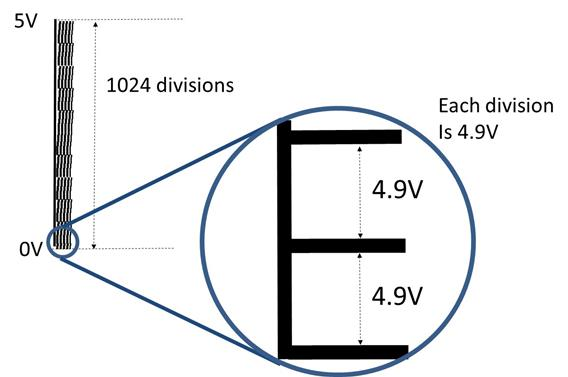
\includegraphics[width=0.8\textwidth]{PH4CAU1M}
\caption[Discretization of voltage measurements on an Arduino]{Discretization
of voltage measurements on an Arduino. The Arduino can measure a range 
of 0-5 Volts, but the digital representation of that measurement is 
stored in a limited number of bits. As a result, the continuous
5 Volt range is chopped up into smaller divisions.}
\label{fig:adc_discretization}
\end{figure} 

Changes in
voltage that are less than $4.9\unit{mV}$ cannot be measured by
an Arduino, since it takes a
whole $4.9\unit{mV}$ to get a different division. So if we give our Arduino $%
8\unit{mV}$ this is not enough to fill the second $4.9\unit{mV}$ division,
so our Arduino would still read only $4.9\unit{mV}.$ If we gave it $11\unit{%
mV}$ it would then read $9.8\unit{mV}$ because $9.8\unit{mV}=2\times 4.9%
\unit{mV}$ and $9.8$ is the closest whole unit of $4.9\unit{mV}.$

%\begin{figure}[h!]
%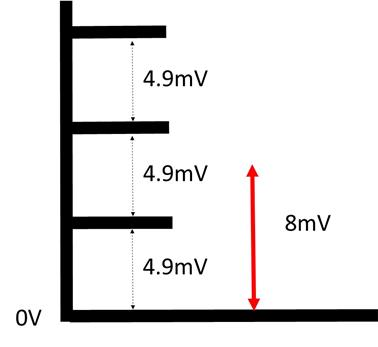
\includegraphics[width=3.1868in,height=2.9265in]{PH4CAU1N}
%\end{figure}%

This is called \textquotedblleft discretization\textquotedblright\ or more
commonly \textquotedblleft digitization\textquotedblright\ or even
\textquotedblleft \emph{quantization.\textquotedblright\ } We have taken a
signal that might have any value between $0$ to $5\unit{V}$ and we output a
signal that will be rounded to the nearest $n\times 4.9\unit{mV}.$

A helpful analogy is to think about a ramp next to a set of stairs. The ramp
is like the analog signal. You can be at any elevation between the bottom and
the top of the ramp. The stairs are like the digital representation of that
signal. There are only discrete elevations that you can obtain. When we convert
an analog signal to a digital signal, we basically just report whatever ``step''
is closest to the analog value.

As a second example, consider using our Arduino to measure a voltage of
$3.793\unit{V}$. We can only measure in steps of 4.9 mV, and if we divide
our voltage by that minimum step size, we get 
\begin{equation*}
\frac{3.793\unit{V}}{4.9\unit{mV}}=774.08
\end{equation*}
The Arduino has to record this ratio as an integer value, so the 0.08 would be
dropped, and the ADC would simply report that the measurement is on step 774,
which corresponds to $774\times4.9\unit{mV}=3.7926\unit{V}$. Similarly, let's 
consider the $4.3276854325532573457\unit{V}$ from our hypothetical power supply.
Following the same method, the Arduino finds that this is closest to ``step'' 
883 in the ADC, which corresponds to 4.3267 Volts. (Make sure you can see how
this result is obtained!)

All of this means that, when we measure voltages with our Arduino, 
we can be off in our voltage measurements as much as $4.9%
\unit{mV}$! In dividing up our voltage range into $1024$ pieces we have
introduced some error, but we have divided our $0$ to $5\unit{V}$ into
numeric values that we can use in our computer, so it is worth the cost of
some error.

The amount of error depends on how many different values the ADC converter
has. Since breaking an analog signal into discrete values is called \emph{%
quantization, }we call this source of error \emph{quantization error.} It is
the source of much of the error we see in electronic measuring devices. We
could say that our new voltmeter has an uncertainty of at least the voltage
resolution%
\begin{equation*}
\delta V_{signal}=\Delta V_{\min }=4.\,\allowbreak 9\unit{mV}
\end{equation*}%
but of course it could be larger if there are other sources of error.

One way to reduce the amount of quantization error in a measurement like this
is to use a data register with more bits. A ten bit register has 1024 
($2^{10}$) discrete
values. A twelve bit register would have $2^{12}=4096$
discrete values. Modern computer chips work with 64 bit registers, which have
$2^{64}=1.845\times10^{19}$ discrete values!

Of course, the only way we could increase the number of bits available on the
Arduino's ADC would be to start replacing physical elements on the Arduino
board. We're not going to attempt that, so we'll just have to live with our
4.9 mV quantization uncertainty.

It's important to note at this point that the ADC does not record the voltage.
Rather, it records which ``step'' the voltage corresponds to. This integer value
is sometimes referred to as an ADC unit.
If we have a signal voltage of $9.8\unit{mV}$, the ADC doesn't provide
us with a ``$9.8$'', but instead it provides a ``2''
because $9.8\unit{mV}=2\Delta V_{\min }.$ The ADC units are the
number of $\Delta V_{\min }$ sized units that are in our signal voltage. To
get back to voltage units, we need to multiply the ADC units 
by $\Delta V_{\min }.$ In our
code we will do this before sending the value to the computer.

\subsection{Sending the Data to the Computer}

The Arduino reads voltage in discrete steps, but can also do further processing
with the ADC values.

Of course, we would like to record the voltage that we measure rather than
the ADC value. There is a
simple way to do this in the Arduino sketch, and that is simply multiplying 
the ADC value by the $\Delta V_{\min}$. 
The voltage values we calculate can be sent to our
computer through the serial cable. We will need an Arduino sketch with some
additional setup and some additional loop commands. One of these commands
will turn our ADC\ units into volts.

Before we look at the entire sketch, let's introduce the new commands that
we will need. To get the Arduino to communicate with the computer we use the
command \code{Serial.begin(9600);} in the setup portion, and 
in the loop function we use the command \code{Serial.print();}. The
\code{Serial.begin(9600);} instructs the Arduino to start sending data out
through the serial port (physically, this is the USB cable that you connect to 
your computer). The \code{9600} argument to this function tells the Arduino
to send this data at 9,600 bits per second (a.k.a. 9,600 baud). (As a side
note, we will be sending text to the serial port in today's activities. The
text characters are represented by an eight digit - or eight bit - binary 
number. Consequently, each text character requires eight bits to be sent to
the serial port.) 

Both ends of the serial communication - in this case our Arduino and the 
computer - need to know what the baud rate is for the communication. If my 
Arduino is sending information at 9,600 bits per second, but my computer is 
only expecting to read 4,800 bits per second, the computer will ``miss'' half 
of the data the Arduino is sending! The serial monitor built into the Arduino 
IDE (which is where we're sending our serial data today) expects data at 
9,600 bits per second, which is why we are sending the information at 
9,600 baud.

The \code{Serial.print()} function translates the 
character string passed as an argument into binary and sends it down the 
serial port pipeline.

We also need to know that computers make a distinction between integer and
real numbers. Our voltages will be real numbers, so we need to tell the
Arduino that we want a real number. The data type for real numbers is the word
\textquotedblleft float.\textquotedblright\ For example,
\code{float delta\_v\_min=0.0049;} 
defines a real number 
variable named \textquotedblleft delta\_v\_min\textquotedblright\
and sets it to the value $0.0049.$ If we want an integer number we use the
data type \textquotedblleft int.\textquotedblright\ For example
\code{int value = 0;}
defines an integer 
variable named \textquotedblleft value\textquotedblright\ and sets
it equal to 0. 

If you are familiar with Python, you know that creating a list of variables
near the beginning of your code is a good idea, not only so you can be sure
that all of your variables are properly initialized, but because it also makes
it a lot easier to decipher your code later on. With the Arduino (as with C or 
C++), if you don't declare your variables up front, the code will not compile, 
and the Arduino software will spit out an error message.

We also need special commands to read our Arduino analog pins. The special
Arduino command \code{analogRead();}  
will do this.

The whole Arduino sketch might look like this:
\lstinputlisting[language=Arduino]{Code/DAQ_voltmeter.ino}

Make sure you understand every line of this code. Write it in the Arduino
IDE and run it to help see what the lines do. Remember that lines that 
begin with two
slashes, \textquotedblleft //,\textquotedblright\ are comments. The Arduino
will ignore these lines, but you shouldn't! The comments tell you, the
programmer, what the code is doing. It's a good habit to include comments
for every line. If there is any part of this sketch that is mysterious, work
with your group to resolve the mystery and if it is still mysterious, call
your instructor over to discuss the sketch with you.

\subsection{Wiring the simple voltmeter}

Now we're ready to build our voltmeter.

\begin{figure*}[h!]
\centering

\includegraphics[width=1.8507in,height=0.9677in]{PH4CAU1O}
\end{figure*}
You knew that was coming, didn't
you? We must be very careful to wire our Arduino correctly. Our Arduino can
measure $0$ to $5\unit{V}.$ But if we switch the $5\unit{V}$ and the $0\unit{%
V}$ by plugging them into the wrong pin, our Arduino will be damaged and
will never work the same way again (probably won't work at all!). So wire
first, then before you connect the Arduino have a group member check your
wiring, then check the wiring with a stand-alone meter (that is why we
learned to use them last time). Also remember, signals of more than 
$5\unit{V}$ (or less than $0\unit{V}$) will 
damage the Arduino. So only put in voltages in the range $0\unit{V}$ to $5%
\unit{V}.$

We need one wire attached to the pin marked A0. We need another wire
attached to one of our Arduino ground pins marked GND. And we connect the
first wire to the positive output of our signal source (say, our power
supply) and the GND wire to our negative output of our signal source (say
the negative or ground connection on our power supply). That is all there is
to it!

\subsection{Seeing the data}

Once the code is compiled and uploaded, the Arduino will send data to the
serial port. The serial monitor can display the data. The serial monitor is
found under the Arduino Software Tools menu 
(Figure \ref{fig:serial_monitor_menu}).

\begin{figure}[htbp!]
\centering
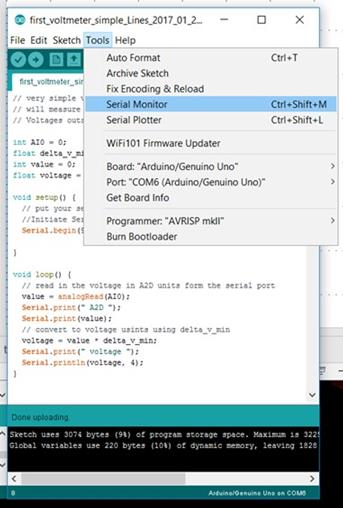
\includegraphics[width=0.5\textwidth]{PH4CAU1P}
\caption[Serial Monitor location in the Arduino IDE]{Serial Monitor
location in the Arduino IDE.}
\label{fig:serial_monitor_menu}
\end{figure}

When activated, the serial monitor will look something like
Figure \ref{fig:serial_monitor}

\begin{figure}[htbp!]
\centering
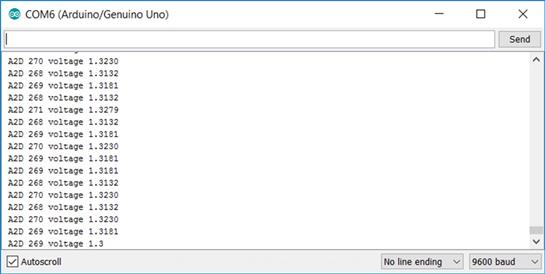
\includegraphics[width=0.8\textwidth]{PH4CAU1Q}
\caption[The Serial Monitor window]{The Serial Monitor window.}
\label{fig:serial_monitor}
\end{figure}

The Arduino Software can also plot the data from the serial port. This is
accessed just below the serial monitor in the Arduino IDE menu.
Figure \ref{fig:serial_plotter} shows a
plot of the same data that we saw in Figure \ref{fig:serial_monitor}. 
In this image, we are plotting both our
voltage values and our ADC values. This makes the voltage
values hard to see (since they are very small, numerically, in comparison
with the ADC values). We could fix this by commenting out the lines that print
the ADC values (putting \textquotedblleft //\textquotedblright\ at the
beginning of the line), so that those lines won't be executed by the Arduino.
Then we get just the voltage (Figure \ref{fig:serial_plotter_2}. 
Notice that the horizontal axis
does not represent the exact time. 
It is just a data point number. We could convert this
to time with some calculation if we know how often the Arduino sends us a
data point. This will be left as an exercise.

\begin{figure}[htbp!]
\centering
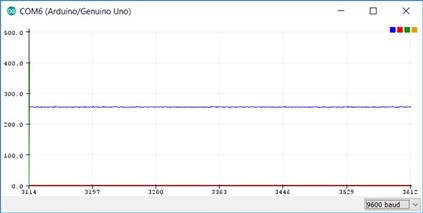
\includegraphics[width=0.8\textwidth]{PH4CAU1R}
\caption[The Serial Plotter window]{The Serial Plotter window.}
\label{fig:serial_plotter}
\end{figure}

\begin{figure}[htbp!]
\centering
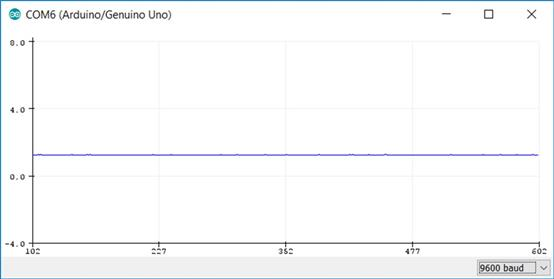
\includegraphics[width=0.8\textwidth]{PH4CAU1S}
\caption[The serial plotter with voltage only]{The serial plotter with
voltage only.}
\label{fig:serial_plotter_2}
\end{figure}

The Arduino is now measuring the voltage (or rather the voltage ADC value),
converting it to usable data, and sending it to our computer! Eventually we will
want to be able to save this data to a file, so it can be used later. That will
be a topic for the next lab period.

\activity
{
Build and use a simple Arduino voltmeter.
\begin{enumerate}
\item Build a circuit with a power supply and a resistor as in 
	Figure \ref{fig:voltage_measurement}. You can choose any resistor. 

\item Write the simple voltmeter sketch.

\begin{center}

\includegraphics[width=1.8507in,height=0.9677in]{PH4CAU20}
\end{center}
\item Wire the Arduino across the resistor, and measure the voltage 
	across the resistor using the Arduino and the serial monitor. 
	Be careful to stay in the $0$ to $5 \unit{V}$ range!

\item Calculate the uncertainty due to quantization error for your Arduino
simple voltmeter

\item Compare your calculated uncertainty to the measured uncertainty that
you see in your device output. (This is tricky, does the power supply give a
truly constant voltage?)
\end{enumerate}

}

\section{Extending our voltmeter with a voltage divider\label{Voltmeter with
Voltage Divider}}

This Arduino-based voltmeter that we have built is great, but will only let
us measure voltages in the range $0$ to $5\unit{V}.$ That seems a little
restrictive. We would like to extend our voltmeter to a larger range, say, $%
0 $ to $20\unit{V}.$ To do this, we will need to add some electronic
components and think about what we have learned about voltage, resistance,
and current. Let's consider the circuit in Figure \ref{fig:voltage_measurement},
which consisted of a battery and a single resistor.
We have a battery, which will make
the current flow much like a pump makes water move through pipes.

\begin{figure}[htbp!]
\centering
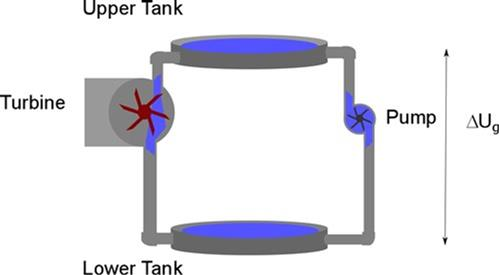
\includegraphics[width=0.8\textwidth]{PH4CAU1U}
	\caption[Water pump analogy for a simple resistor circuit]{Water pump
	analogy for a simple resistor circuit. The pump and the battery play 
	the same role.}
	\label{fig:water_pump_analogy_1}
\end{figure}

The water in a pipe system (Figure \ref{fig:water_pump_analogy_1}) gains
potential energy as it moves up. In our circuit we will find that electric
charge gains potential energy as we move it across a battery. Then the
charge will move down the wire like water moves down a pipe until it is out
of potential energy. Notice that the water in a pipe system will lose all
the potential energy that it gained when the pump raised it to the upper
tank (see Figure \ref{fig:water_pump_analogy_1}). 
That is true of electric charge too. The
electric current travels from the battery through the resistor, but in doing
so it loses all the potential energy that the battery gave it by the time it
returns to the battery.

Now suppose we have two resistors in a circuit, as in Figure
\ref{fig:voltage_divider}. 

\begin{figure}[htbp!]
\centering
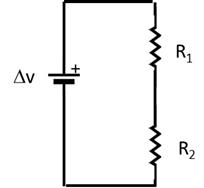
\includegraphics[width=0.3\textwidth]{PH4CAU1V}
\caption[A two-resistor circuit]{A two-resistor circuit. The two 
resistors in series are also called a voltage divider.}
\label{fig:voltage_divider}
\end{figure}

Our water analogy can still help us understand what will happen. Suppose
that we have two turbines in our pipe system, as in Figure
\ref{fig:water_pump_analogy_2}
The water leaves the high
potential energy part of the pump, and is put to work turning the first
turbine. The resistance of the turbine will slow the water current. So when
the water leaves the turbine, it will have lost some potential energy. Since
we have a second turbine the current will again be slowed and more potential
energy will be lost. How much potential energy do we lose as the water
falls? All of the potential energy that the pump gave it! We must end up
with the water at the bottom back at the low potential energy. We will find
this to be true for our electric circuit as well. We will lose some
potential energy as the electrical energy \textquotedblleft
falls\textquotedblright\ from the high electric potential \textquotedblleft
down\textquotedblright\ the first resistor. After the second resistor, we
can guess that we must be back at the low electric potential we started with.
\begin{figure}[htbp!]
\centering
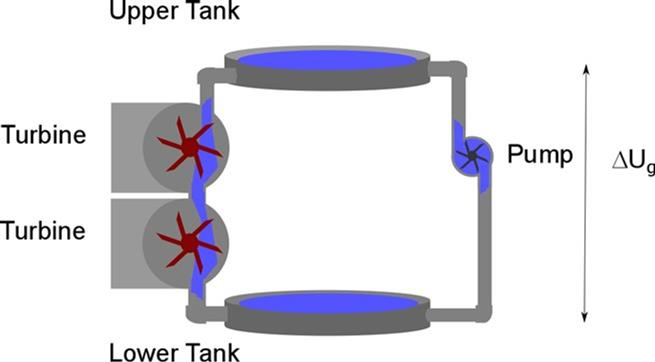
\includegraphics[width=0.8\textwidth]{PH4CAU1W}
\caption[A water pump system with two turbines]{A water pump system
with two turbines, analogous to a two resistor circuit.}
\label{fig:water_pump_analogy_2}
\end{figure}

In summary, the electric potential supplied by a battery (or any other source
of potential) will be entirely ``used up'' by the time the current goes through 
the entire circuit. When I have two resistors in series with a battery, as in 
\ref{fig:voltage_divider}, only part of the potential is used up in the first 
resistor, and the rest is used up in the second resistor. Consequently, if our
power source was a 9.0 V battery, and the two resistors had equal resistance, 
the potential would only drop 4.5 V in the first resistor, and then the 
remaining 4.5 volts in the second resistor. We have effectively divided a 
(larger) voltage into two smaller parts, and consequently these two 
resistors in series are known as a \textbf{voltage divider}.

Note that you don't have to use two resistors with equal resistance in a 
voltage divider. The fraction of the voltage ``used up'' in each resistor 
ends up being proportional to the resistance (in comparison with the total
resistance) as we will see. For example, if we had a 30 V power source (more 
than sufficient to send our Arduino to the scrap bin) combined with a 
voltage divider consisting of a 1000 Ohm resistor and 5000 Ohm resistor,
the total resistance would be 6000 Ohms. The fraction of the voltage that 
will be used up in the first 1000 Ohm resistor is (1000 Ohm)/(6000 Ohm), or
1/6. 1/6 of 30 V is 5 V - a potential difference that is safe for our Arduino!
The remaining 25 V of potential will be used up across the 5000 Ohm resistor.

Let's take a look at the math in a little more detail.

We know that electric potential
is a potential energy per unit charge, and energies just add up. If 
\begin{equation*}
\Delta V=RI
\end{equation*}%
is satisfied, then we would expect that adding two resistors would just
linearly add the effects of the two resistors together%
\begin{eqnarray*}
\Delta V_{total} &=&\Delta V_{1}+\Delta V_{2} \\
&=&R_{1}I+R_{2}I
\end{eqnarray*}%
Note that the same current must flow through each of the resistors, since
the current leaving $R_{1}$ is the current flowing into $R_{2}.$ Then 
\begin{equation*}
\Delta V_{total}=\left( R_{1}+R_{2}\right) I
\end{equation*}%
Our current will be 
\begin{equation*}
I=\frac{\Delta V_{total}}{R_{1}+R_{2}}
\end{equation*}

\begin{figure}[htbp!]
\centering
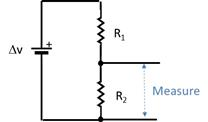
\includegraphics[width=0.3\textwidth]{PH4CAU1Y}
\caption[Measuring voltage in a voltage divider]{Measuring voltage in a
voltage divider.}
\label{fig:voltage_divider_2}
\end{figure}
But suppose we measure the potential change across just resistor $R_{2}$, as
in Figure \ref{fig:voltage_divider_2}.
What would we expect to get? We
lost voltage across both $\Delta V_{1}$ and $\Delta V_{2}$ so 
\begin{equation*}
\Delta V_{total}=\Delta V_{1}+\Delta V_{2}
\end{equation*}%
because we must lose all the $\Delta V_{total}$ given to the current by the
battery. And 
\begin{equation*}
\Delta V_{2}=IR_{2}
\end{equation*}%
from Ohm's law. So
\begin{equation*}
\Delta V_{2}=\left( \frac{\Delta V_{total}}{R_{1}+R_{2}}\right) R_{2}
\end{equation*}%
This is only part of the total voltage, and if we have two different
resistors so that $R_{1}\neq R_{2}$ then we can choose for $\Delta V_{2}$ to
be nearly as much as $\Delta V_{total}$ or nearly as little as $0$ by
carefully choosing our two resistances. We call a set of two resistors like
this a \textquotedblleft voltage divider\textquotedblright\ because it
divides the battery voltage between the two resistors. If $R_{1}$ is bigger
than $R_{2}$ then $\Delta V_{1}$ is bigger than $\Delta V_{2}.$

Remember that the input can only withstand $0$ to $5\unit{V}.$ More than
that can destroy the board! But we want to measure a voltage that varies
from $0$ to $20\unit{V}.$ We now have a way to do this. We will use a
voltage divider. The voltage across both resistors will be as much as $20%
\unit{V},$ but we will measure the voltage across only one of the resistors.
We will choose our resistor so that when the total voltage is $20\unit{V}
$ but the voltage across our resistor is $5\unit{V}$ (or less). Since we
will know the resistances, we can use a little math to calculate what the
total voltage was using the voltage measurement from just one of the
resistors.

This is like what we did to measure current last lab. We used a voltmeter
and a resistor and some math to make an ammeter. Today we will use two
resistors, our Arduino voltmeter, and some math to make a new voltmeter that
can measure higher voltages. We just need to choose our resistors so that we
map our $0$ to $20\unit{V}$ to $0$ to $5\unit{V}.$ Once choice might be 
\begin{eqnarray*}
R_{1} &=&40\unit{k%
%TCIMACRO{\U{3a9}}%
%BeginExpansion
\Omega%
%EndExpansion
} \\
R_{2} &=&10\unit{k%
%TCIMACRO{\U{3a9}}%
%BeginExpansion
\Omega%
%EndExpansion
}
\end{eqnarray*}%
Let's try it. We would get%
\begin{eqnarray*}
\Delta V_{2\max } &=&\left( \frac{20\unit{V}}{40\unit{k%
%TCIMACRO{\U{3a9}}%
%BeginExpansion
\Omega%
%EndExpansion
}+10\unit{k%
%TCIMACRO{\U{3a9}}%
%BeginExpansion
\Omega%
%EndExpansion
}}\right) \left( 10\unit{k%
%TCIMACRO{\U{3a9}}%
%BeginExpansion
\Omega%
%EndExpansion
}\right) \\
&=&4.0\unit{V}
\end{eqnarray*}%
when $\Delta V_{total}=20\unit{V}$ and 
\begin{eqnarray*}
\Delta V_{2\min } &=&\left( \frac{0\unit{V}}{40\unit{k%
%TCIMACRO{\U{3a9}}%
%BeginExpansion
\Omega%
%EndExpansion
}+10\unit{k%
%TCIMACRO{\U{3a9}}%
%BeginExpansion
\Omega%
%EndExpansion
}}\right) \left( 10\unit{k%
%TCIMACRO{\U{3a9}}%
%BeginExpansion
\Omega%
%EndExpansion
}\right) \\
&=&0\unit{V}
\end{eqnarray*}%
when $\Delta V_{total}=0\unit{V}.$ Notice that this really didn't work. We
only got a maximum voltage of $4\unit{V}.$ But this gives us a margin of
safety. If we give our Arduino more than $5\unit{V}$ we can burn it up. If
we plan our circuit so we don't get too close to $5\unit{V}$ we are safer. So
this set of resistors is not a terrible choice.

To report out our voltage we need to do this conversion backwards. Say we
have $\Delta V_{total}=10\unit{V}$ that we are measuring with our new
instrument. Then 
\begin{eqnarray*}
\Delta V_{2} &=&\left( \frac{10\unit{V}}{40\unit{k%
%TCIMACRO{\U{3a9}}%
%BeginExpansion
\Omega%
%EndExpansion
}+10\unit{k%
%TCIMACRO{\U{3a9}}%
%BeginExpansion
\Omega%
%EndExpansion
}}\right) \left( 10\unit{k%
%TCIMACRO{\U{3a9}}%
%BeginExpansion
\Omega%
%EndExpansion
}\right) \\
&=&2\unit{V}
\end{eqnarray*}

The $2\unit{V}$ is what we actually measure at the A0 input. But we know
that this represents $10\unit{V}$ across both resistors, so we want the
Arduino program to print out $10\unit{V}.$ So we report%
\begin{equation*}
\Delta V_{reported}=\frac{\Delta V_{2}}{R_{2}}\left( R_{1}+R_{2}\right)
\end{equation*}%
or for our case, since we measured $2\unit{V}$ across our resistor,%
\begin{equation*}
10\unit{V}=\frac{2\unit{V}}{\left( 10\unit{k%
%TCIMACRO{\U{3a9}}%
%BeginExpansion
\Omega%
%EndExpansion
}\right) }\left( 40\unit{k%
%TCIMACRO{\U{3a9}}%
%BeginExpansion
\Omega%
%EndExpansion
}+10\unit{k%
%TCIMACRO{\U{3a9}}%
%BeginExpansion
\Omega%
%EndExpansion
}\right)
\end{equation*}%
We will have to write this math in our code. 

There is a further
complication. The Arduino A0 input is giving us a number that represents $0$
to $4\unit{V}$ for our setup. But that is not what we see on the serial
port. We see a number from 0 to 1024. We know the $1024$ represents $5\unit{V%
}$ and the $0$ represents $0\unit{V}.$ So we need to multiply the number
that comes from our Arduino by $\delta V=4.9\unit{mV}$ once again to get our
Arduino output into voltage units. So our reported voltage equation is
something like this. 
\begin{equation*}
\Delta V_{reported}=A2D\times \delta V_{2}\times \frac{1}{R_{2}}\left(
R_{1}+R_{2}\right)
\end{equation*}

All this calculation to get our reported voltage must do something to our
measurement uncertainty. We could do our usual math to find the reported
uncertainty, but instead, let's think. Every small voltage $\Delta V_{2}$
would be multiplied by $\left( \frac{1}{R_{2}}\left( R_{1}+R_{2}\right)
\right) $ to map it into our original $0\unit{V}$ to $20\unit{V}$ range.
That should work for our smallest voltage that we can detect, namely $\delta
V=4.9\unit{mV}.$ That is the smallest value $\Delta V_{2}$ could have. So in
our $0\unit{V}$ to $20\unit{V}$ range the smallest value this can map to is 
\begin{equation*}
\delta V_{reported}=\left( \delta V\right) \left( \frac{1}{R_{2}}\left(
R_{1}+R_{2}\right) \right)
\end{equation*}%
The first term in parenthesis is essentially $1$ digitizer unit multiplied
by $\Delta V_{2}$ and the second term in parenthesis converts the $\Delta
V_{2}$ value into actual volts measured across both resistors.

The quantity $\delta V_{reported}$ gives us our quantization error value for
our new instrument. Our output will be in multiples of 
\begin{equation*}
V_{reported}=n\times \delta V_{reported}
\end{equation*}%
Putting in numbers gives 
\begin{eqnarray*}
\delta V_{reported} &=&\left( 4.\,\allowbreak 884\times 10^{-3}\unit{V}%
\right) \left( \frac{1}{10\unit{k%
%TCIMACRO{\U{3a9}}%
%BeginExpansion
\Omega%
%EndExpansion
}}\left( 40\unit{k%
%TCIMACRO{\U{3a9}}%
%BeginExpansion
\Omega%
%EndExpansion
}+10\unit{k%
%TCIMACRO{\U{3a9}}%
%BeginExpansion
\Omega%
%EndExpansion
}\right) \right) \\
&=&0.024\,42\unit{V} \\
&=&24.42\unit{mV}
\end{eqnarray*}%
This is much bigger than our $4.9\unit{mV}$ uncertainty for the simple
voltmeter. This is the cost of using a voltage divider to extend our
voltage range. For the bigger voltage range we get a bigger uncertainty.

Let's try another example. Suppose we wish to measure $0$ to $20\unit{V}$
and we look in our case of resistors and find we have the following two
resistors to use:%
\begin{eqnarray*}
R_{1} &=&98\unit{k%
%TCIMACRO{\U{3a9}}%
%BeginExpansion
\Omega%
%EndExpansion
} \\
R_{2} &=&15\unit{k%
%TCIMACRO{\U{3a9}}%
%BeginExpansion
\Omega%
%EndExpansion
}
\end{eqnarray*}

We would expect that our $0$ to $20\unit{V}$ would be mapped to a smaller
range. Let's find that range.%
\begin{eqnarray*}
\Delta V_{2\max } &=&\left( \frac{20\unit{V}}{98\unit{k%
%TCIMACRO{\U{3a9}}%
%BeginExpansion
\Omega%
%EndExpansion
}+15\unit{k%
%TCIMACRO{\U{3a9}}%
%BeginExpansion
\Omega%
%EndExpansion
}}\right) \left( 15\unit{k%
%TCIMACRO{\U{3a9}}%
%BeginExpansion
\Omega%
%EndExpansion
}\right) \\
&=&2.\,\allowbreak 654\,9\unit{V}
\end{eqnarray*}%
So our voltage range at the Arduino A0 input will be $0\unit{V}$ to $%
2.\,\allowbreak 65\unit{V}.$ This set of resistors won't use the full
Arduino $0\unit{V}$ to $5\unit{V}$ range. But it will measure $0$ to $20%
\unit{V}.$ The minimum detectable voltage for this new instrument design for
our $0$ to $20\unit{V}$ source will be 
\begin{eqnarray*}
\delta V_{reported} &=&\left( \delta V_{2}\right) \left( \frac{1}{R_{2}}%
\left( R_{1}+R_{2}\right) \right) \\
&=&\left( 4.\,\allowbreak 880\,3\times 10^{-3}\unit{V}\right) \left( \frac{1%
}{\left( 15\unit{k%
%TCIMACRO{\U{3a9}}%
%BeginExpansion
\Omega%
%EndExpansion
}\right) }\left( 98\unit{k%
%TCIMACRO{\U{3a9}}%
%BeginExpansion
\Omega%
%EndExpansion
}+15\unit{k%
%TCIMACRO{\U{3a9}}%
%BeginExpansion
\Omega%
%EndExpansion
}\right) \right) \\
&=&3.\,\allowbreak 676\,5\times 10^{-2}\unit{V} \\
&=&37\unit{mV}
\end{eqnarray*}

This uncertainty is much bigger than the uncertainty for our last choice of
resistors. So $98\unit{k%
%TCIMACRO{\U{3a9}}%
%BeginExpansion
\Omega%
%EndExpansion
}$ and $15\unit{k%
%TCIMACRO{\U{3a9}}%
%BeginExpansion
\Omega%
%EndExpansion
}$ are not great choices even though they technically work.

For your version of the voltmeter in lab, you will choose the resistor
values to use. Here is an Arduino sketch to implement this extended volt
meter. In it are the not-so-good $98\unit{k%
%TCIMACRO{\U{3a9}}%
%BeginExpansion
\Omega%
%EndExpansion
}$ and $15\unit{k%
%TCIMACRO{\U{3a9}}%
%BeginExpansion
\Omega%
%EndExpansion
},$ but of course \textbf{you should change the sketch to have your resistor
values}.
\lstinputlisting[language=Arduino]{Code/DAQ_Extended_voltmeter.ino}


\bigskip Of course you will want to have another person check your math and
wiring, and you should check your output voltage with a stand-alone meter
before you plug into your Arduino.

\section{Practice Problems}

Here is an example for you to work out on your own before class. Do this and
compare your result to the results of the other people in your lab group as
you come into class on lab day.

Suppose we wish to measure $0$ to $15\unit{V}$ and we look in our case of
resistors and find we have the following two resistors to use:%
\begin{eqnarray*}
R_{1} &=&43.2\unit{k%
%TCIMACRO{\U{3a9}}%
%BeginExpansion
\Omega%
%EndExpansion
} \\
R_{2} &=&15.2\unit{k%
%TCIMACRO{\U{3a9}}%
%BeginExpansion
\Omega%
%EndExpansion
}
\end{eqnarray*}%
What range of voltages would we see at the Arduino, and what is the
quantization error for our measurement?

\clearpage
\activity
{
Build an extended voltmeter using a voltage divider.

\begin{enumerate}
\item Build the voltage divider using two resistors as described in Section
\ref{Voltmeter with Voltage Divider}. You will have to think about which
resistors from our set will work best. Discuss this with your group, or have
group members try the calculations with different combinations.

\item Use a multimeter to verify that the output of the voltage divider is
never more than $5\unit{V}$ and never less than $0\unit{V}.$ Take your power
supply all the way from $0\unit{V}$ to $20\unit{V}$ (or whatever
the maximum of the power supply is) and watch the multimeter
to ensure it stays in the $0$ to $5\unit{V}.$ range.\textbf{\ Do this with a
multimeter before you hook up your Arduino.} You are making sure everything
works so you won't destroy your Arduino!

\begin{center}

\includegraphics[width=1.8507in,height=0.9677in]{PH4CAU21}
\end{center}
\item Write the sketch and then hook
the output of your voltage divider to the A0 pin and the other side of $%
R_{2} $ to a GND pin.
Your voltmeter should now be set
up. Compile and load the sketch and use the Serial Plotter to watch the
voltage values as you take the power supply from $0$ to $20\unit{V}$ using
the serial monitor or plotter.

\item What is the quantization error for this voltmeter? Check to see if
	this matches your values on the serial monitor. (The values on the
		serial monitor should ``jump'' in steps with a size equal to
		the quantization error).
\end{enumerate}
}
